% PLANO DE TRABALHO-------------------------------------------------------------------

\chapter{PLANO DE TRABALHO}
\label{chap:planoDeTrabalho}

Na seção deste capítulo é apresentado o cronograma e as atividades desenvolvidas durante um determinado período para que a execução do projeto se conclua.

\section{CRONOGRAMA}

\begin{figure}[!htb]
    \centering
    \caption{Cronograma das atividades}
    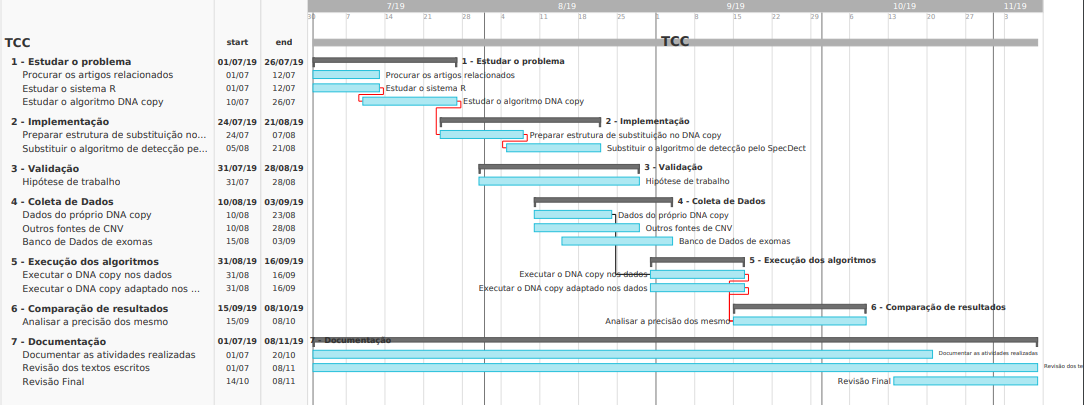
\includegraphics[width=1\textwidth]{./dados/figuras/Figure-3-TCC}
    \fonte{Autoria Própria}
    \label{fig:figure-3-TCC}
\end{figure}

\subsection{ATIVIDADES DO CRONOGRAMA}

O cronograma para o desenvolvimento do projeto apresenta um conjunto de sete grupos de atividades, contendo atividades pequenas aninhada em torno de sua atividade raiz como visto na \autoref{fig:figure-3-TCC}. A seguir encontra-se uma descrição do maior grupo de atividades a serem executadas neste projeto:

\begin{enumerate}
   \item Estudar o problema
   \begin{description}
        \item Investigação do assunto referente ao problema, buscando o entendimento de \textit{Change Point} e a aplicação de algoritmos de segmentação, \textit{Copy Number Variation}, linguagem R e a estrutura do DNAcopy.
    \end{description}
   \item Implementação
   \begin{description}
        \item Desenvolvimento da estrutura para criação do projeto proposto, efetivando o objetivo proposto no trabalho.
    \end{description}
   \item Validação
   \begin{description}
        \item Estudo e preparação para o algoritmo trabalhado, buscando o analise da estrutura para que a validação seja feita.
    \end{description}
   \item Coleta de Dados
   \begin{description}
        \item Busca por dados a serem utilizados como teste no projeto criado e em trabalhos de comparação com mesmo.
    \end{description}
   \item Execução dos algoritmos
   \begin{description}
        \item Execução e coleta de dados gerados a partir dos testes realizados nos trabalhos selecionados anteriormente
    \end{description}
   \item Comparação dos resultados
   \begin{description}
        \item Análise dos dados da aplicação dos algoritmos testados de acordo com a Matriz de Confusão descrita no \autoref{chap:metodologia}
    \end{description}
   \item Documentação
   \begin{description}
        \item Levantamento da escrita sobre as atividades realizadas e dados obtidos com o desenvolvimento do projeto.
    \end{description}
 \end{enumerate}